
As stated in our introduction, we aim to answer how different groups in our string taxonomy differ in their 
characteristics (RQ2).
Therefore we analyzed string columns from Kaggle, Huggingface, IMDB and Stackoverflow.
For each column, we compute the count, null count, empty count, distinct count, length percentiles, a value histogram, a char histogram
and more, which is available in DBPile's \texttt{column\_stats\_text} table.

In DBMS storage engines and analytical file formats such as Parquet \cite{NEEDED}, values are stored
and compressed in row groups of a fixed size.
All statistics in this work are computed at the level of a single row group.
For this paper, we assume a row group size of 122,880 values, which corresponds to the default configuration used by DuckDB.
As these statistics also correlate with compressibility, we want to have the same methodology in retrieving the column stats as the compression results.

\begin{figure}[h!]
  \centering
\begin{subfigure}{0.35\linewidth}
   \centering
  
\includegraphics[width=\linewidth]{assets/string_stats/duplicates/TPC/All_duplicates.pdf}
  \caption{TPC-[H/DS]}
  \label{fig:string_properties_dups_tpc_vs_others:all_duplicates}
\end{subfigure}
\begin{subfigure}{0.35\linewidth}
   \centering
  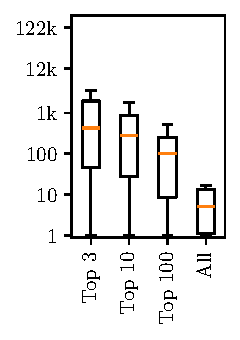
\includegraphics[width=\linewidth]{assets/string_stats/duplicates/Other/All_duplicates.pdf}
  \caption{Other}
  \label{fig:string_properties_dups_tpc_vs_others:all_duplicates}
\end{subfigure}
  \label{fig:string_properties_dups_tpc_vs_others}
  \caption{Duplicate value rates for TPC-[H/DS] datasets vs. all other datasets.}
\end{figure}

First, we examine how many duplicates string columns contain and how these duplicates are distributed. 
For this, we only considered columns with at least 122{,}880 values. Duplicate empty or null values 
do not count as duplicates. We omitted columns from the TPC schema, as they are known to follow a 
uniform distribution that does not reflect real-world data~\cite{NEEDED}. This also applies to TPC string 
columns, as shown in \cref{fig:string_properties_dups_tpc_vs_others}.

The figure shows that real-world datasets have both a more skewed value distribution and fewer duplicates on 
average than TPC columns. This aligns with our taxonomy results: 33\% of TPC columns are categorical, 
compared to an average of 20\%, and categorical columns naturally exhibit more duplicates.

Todo: cite https://link.springer.com/chapter/10.1007/978-3-642-32627-1_10 (Skewed TPC)

\insight{Strings in real-world datasets contain less duplicates but are more skewed than those in TPC datasets.}

\begin{figure*}[h!]
  \centering
\begin{subfigure}{0.1583\linewidth}
   \centering
  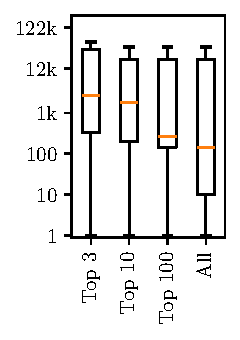
\includegraphics[width=\linewidth]{assets/string_stats/duplicates/Other/Category_duplicates.pdf}
  \caption{Category}
  \label{fig:string_properties_dups:category_duplicates}
\end{subfigure}
\begin{subfigure}{0.1583\linewidth}
   \centering
  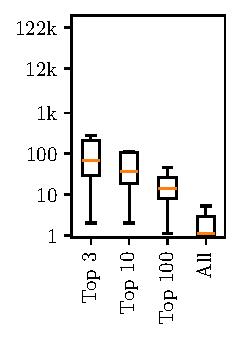
\includegraphics[width=\linewidth]{assets/string_stats/duplicates/Other/Entity_duplicates.pdf}
  \caption{Entity}
  \label{fig:string_properties_dups:entity_duplicates}
\end{subfigure}
\begin{subfigure}{0.1583\linewidth}
   \centering
  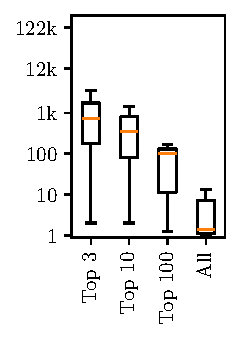
\includegraphics[width=\linewidth]{assets/string_stats/duplicates/Other/FullText_duplicates.pdf}
  \caption{FullText}
  \label{fig:string_properties_dups:fulltext_duplicates}
\end{subfigure}
\begin{subfigure}{0.1583\linewidth}
   \centering
  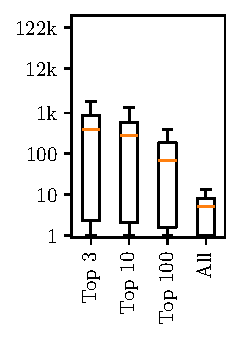
\includegraphics[width=\linewidth]{assets/string_stats/duplicates/Other/Identifier_duplicates.pdf}
  \caption{Identifier}
  \label{fig:string_properties_dups:identifier_duplicates}
\end{subfigure}
\begin{subfigure}{0.1583\linewidth}
   \centering
  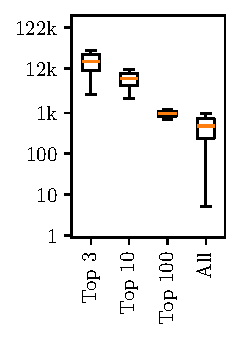
\includegraphics[width=\linewidth]{assets/string_stats/duplicates/Other/Numeric_duplicates.pdf}
  \caption{Numeric}
  \label{fig:string_properties_dups:numeric_duplicates}
\end{subfigure}
\begin{subfigure}{0.1583\linewidth}
   \centering
  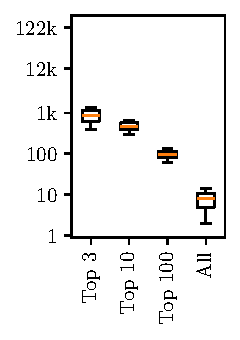
\includegraphics[width=\linewidth]{assets/string_stats/duplicates/Other/Structured_duplicates.pdf}
  \caption{Structured}
  \label{fig:string_properties_dups:structured_duplicates}
\end{subfigure}
  \label{fig:string_properties_dups}
  \caption{Duplicates per row group (122,880 values) per semantic types for all columns excluding TPC-[H/DS] datasets. Only strings that are not null or empty are considered.}
\end{figure*}

That categorical values contain many duplicates is also confirmed by \cref{fig:string_properties_dups}, 
which shows the number of duplicates for different groups in our taxonomy. The figure shows duplicates 
per row group of 122{,}880 for the top 3, 10, and 100 most frequent values, compared to the duplicates across all values.

Categorical columns have the highest duplicate ratios, with a median of 6 duplicates. 
Unlike the other groups, categorical columns show similar duplicate counts for the top 10 and top 100 values. 
This is because they have on average only 12864 distinct values, meaning that the top 10
already includes nearly all values for most columns.

Groups in which a substantial share of columns contain no duplicates include FullText and Identifier columns,
 and to some extent Entities. However, all of these groups still show notable amounts of duplication overall. 
 For Entities, this is expected, since values such as names come from a finite domain. For Identifiers, duplicates 
 can arise from foreign key relationships. For FullText columns, however, duplication is unexpected. Further 
 analysis shows that duplicates in FullText columns occur mainly in Kaggle and Huggingface datasets used for ML 
 applications.

\begin{figure*}[h!]
  \centering
\begin{subfigure}{0.15\linewidth}
   \centering
  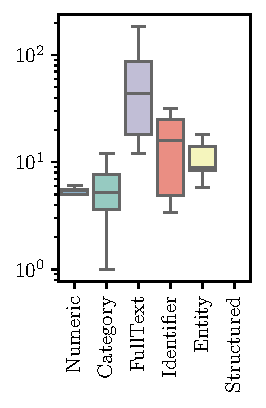
\includegraphics[width=\linewidth]{assets/string_stats/avg_length.pdf}
  \caption{avg. length}
  \label{fig:string_properties:avg_length}
\end{subfigure}
\begin{subfigure}{0.15\linewidth}
   \centering
  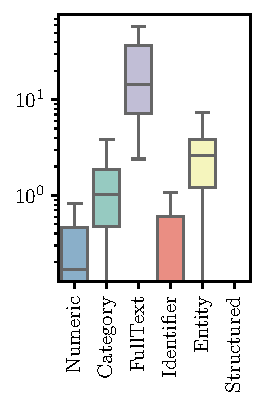
\includegraphics[width=\linewidth]{assets/string_stats/stddev_length.pdf}
  \caption{std. dev. length}
  \label{fig:string_properties:stddev_length}
\end{subfigure}
\begin{subfigure}{0.15\linewidth}
   \centering
  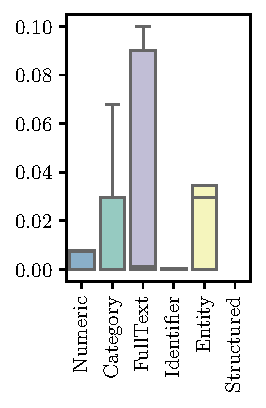
\includegraphics[width=\linewidth]{assets/string_stats/empty_or_null_rate.pdf}
  \caption{\% null or empty }
  \label{fig:string_properties:empty_or_null_rate}
\end{subfigure}
\begin{subfigure}{0.15\linewidth}
   \centering
  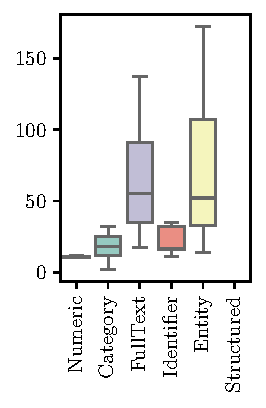
\includegraphics[width=\linewidth]{assets/string_stats/count_unfiltered.pdf}
  \caption{\# distinct chars}
  \label{fig:string_properties:count_unfiltered}
\end{subfigure}
  \label{fig:string_properties}
  \caption{String properties per semantic type for columns with at least 10,000 rows (n=330).}
\end{figure*}

In \cref{fig:string_properties}, we analyze the length and character distribution of different groups in our taxonomy.
We can see that the length of a string varies significantly between groups. FullText columns have the highest lengths,
and also the standard deviation of lengths. Categorical columns, on the other hand, have are often short, 
with 0.0\% having only one character, representing flags or codes. 

Identifier columns are longer, with a average length of 17.2 characters.
However, the standard deviation of lengths for Identifiers is relatively low, with 
41.2\% of columns having all identifier values of the same length. 
The reason for this is mainly uuid identifiers with the top three most common fixed-lengths being 32 (86\%) and 36 (14\%). 
Note that this exceeds both the 12 inline bytes permitted for German strings~\cite{neumann_umbra_2020} and the 16 
bytes that a \texttt{compact\_str}~\cite{timmerman_parkmycarcompact_str_2025} like implementation would inline. 
This also suggests execution-level opportunities: for instance, hashing logic for variable-length 
strings could employ a specialized fast path for these fixed-length identifiers. This shows that there is optimization
potential, such as a specialized hashing path for fixed-length identifiers stored as variable-length strings.

\insight{Different groups in our taxonomy exhibit distinct properties. E.g. identifiers are often 
uniform in length, categorical values are often short, and full text is highly variable. This offers possibilities for type-aware optimizations.}